% TAPLab TRB Annual Meeting paper (2027 requirements). Full draft.
% Compile: pdflatex main.tex (twice).
\documentclass[11pt]{article}
\usepackage[margin=1in]{geometry}
\usepackage{times}
\usepackage{graphicx}
\usepackage{booktabs}
\usepackage{setspace}
\usepackage{lineno}
\usepackage[hidelinks]{hyperref}
\usepackage{caption}
\usepackage{amsmath}
\captionsetup{font=small,labelfont=bf}
\setlength{\parskip}{4pt}
\setlength{\parindent}{0pt}
\newcommand{\citepara}[1]{(#1)}

\begin{document}

% ---------------------------------------------------------------- title page
\begin{center}
{\Large\bfseries TAPLab: An Open Laboratory for Reproducible Traffic
Assignment Experiments}\\[6pt]
{\large Design Principles, Independent Certification, and Cross-Solver
Evidence}\\[18pt]
\end{center}

\textbf{Xuesong (Simon) Zhou, Ph.D.} (Corresponding Author)\\
Professor, School of Sustainable Engineering and the Built Environment\\
Arizona State University, Tempe, AZ 85281\\
Email: xzhou74@asu.edu\\[8pt]
[Co-authors to be added with job titles and affiliations]\\[16pt]

Word count: approximately 7{,}100 words + 8 tables $\times$ 250 = 9{,}100
word equivalents\\
Total number of pages: [to update at submission]\\[8pt]
Submitted for presentation at the Transportation Research Board Annual
Meeting and publication in Transportation Research Record.\\[8pt]
\textit{Disclosure: generative AI tools were used to assist code
development, experiment orchestration, and manuscript drafting under full
author direction and review; all algorithmic designs, definitions, and
conclusions are the authors'.}

\newpage
% ------------------------------------------------- structured abstract page
\section*{Abstract}
\textbf{Objectives.} Computational comparisons of traffic assignment
algorithms are difficult to trust and to reproduce: solvers report their own
convergence measures, interchange-format conversions silently alter the
problem being solved, and results obtained on restricted path pools are
presented as network equilibria. This paper introduces TAPLab, an open
laboratory whose goal is to make traffic assignment experiments
reproducible, independently verifiable, and comparable across solvers,
formats, and modeling systems.

\textbf{Methods.} TAPLab combines four elements: (i) a compact
GMNS-compatible exchange representation in which zones are centroid rows of
the node table and connectors are typed links; (ii) TAPForge, a parametric
instance generator whose manifests record every parameter and seed, so each
instance reproduces from its manifest alone; (iii) a registry of solver
adapters spanning link-based, bush-based, origin-based, path-based, and
compressed-path algorithms drawn from five independent codebases; and
(iv) an independent certification pipeline that recomputes link costs, the
Beckmann objective, node-level flow conservation, and the shortest-path
relative gap from each solver's returned flows, and additionally requires
consistency with the solver's self-reported gap.

\textbf{Findings.} The certification pipeline exposed five latent defects in
standard interchange practice, each invisible to self-reported convergence:
among them, a first-through-node default that let equilibrium paths route
through zone centroids (72\% flow error at a self-reported gap of
$5\times10^{-7}$) and a connector capacity that collided with a solver's
internal artificial-arc sentinel, silently deleting all connector flows.
A certified seven-algorithm comparison across analytical, route-rich,
space--time, and canonical networks confirms that bush-based methods
dominate one-shot equilibrium computation, quantifies a sharp degradation
of an origin-based method on route-rich congested grids, and isolates ---
with the routing kernel held fixed --- when and why path-space compression
pays.

\textbf{Novelty.} TAPLab is, to the authors' knowledge, the first traffic
assignment platform in which every published number carries an independent
certificate, every failure remains visible in the result tables, and every
generated instance is reproducible from its recorded manifest.

\textbf{Practical Applications.} Public agencies can verify vendor solver
claims from returned flows alone; researchers can attribute performance
differences to algorithms rather than implementations; solver developers
obtain a regression laboratory with transparent failure reporting.

\newpage
\linenumbers
% ---------------------------------------------------------------- body
\section{Introduction}

Static traffic assignment remains the computational core of regional travel
models, corridor studies, pricing analyses, and network design. Over five
decades the algorithmic landscape has broadened from link-based convex
combinations --- Frank--Wolfe and its conjugate and biconjugate
accelerations --- to path-based gradient projection
\citepara{Jayakrishnan et al. 1994}, origin- and bush-based equilibration in
the lineage of Bar-Gera's origin-based algorithm and Dial's Algorithm B
\citepara{Bar-Gera 2002; Dial 2006}, paired-alternative-segment methods
such as TAPAS, local user-cost equilibrium (LUCE) \citepara{Gentile 2014},
and, recently, compressed-path representations that carry a low-dimensional
latent structure inside the convex assignment program
\citepara{Zhou et al. 2026}.

Yet the computational evidence on which practitioners choose among these
algorithms is fragile in three specific and recurring ways.

\textbf{First, self-reported convergence.} Nearly every published
comparison ranks solvers at each solver's \emph{own} stopping rule and
\emph{own} gap definition. Relative gap, average excess cost, and objective
improvements are computed inside the solver whose performance is being
judged. When the network the solver actually solved differs from the
network the experimenter intended --- for any of the interchange reasons
below --- the self-reported gap remains perfectly plausible while the
returned flows answer a different question.

\textbf{Second, conversion drift.} Comparisons across solvers require
format conversions (GMNS, TNTP, native binary layouts), and each conversion
is an opportunity to alter the problem silently: centroid-passage rules,
per-lane versus total capacity, authoritative free-flow times versus
length-over-speed reconstructions, numeric precision of exported
parameters, and parser conventions on record ordering. Section~5 documents
five such defects found in widely used, well-tested software, every one of
them invisible to self-reported convergence.

\textbf{Third, restricted-pool conflation.} Path-based and column-based
methods often operate on a working set of routes. A small restricted-master
gap proves that the current pool was optimized well; it does not prove the
pool is adequate. Reporting a pool gap as a network equilibrium claim
conflates two different mathematical statements, and the difference is not
small: in our experiments, pools solved to $10^{-5}$ internal gaps leave
network gaps up to $5.5\times10^{-3}$.

These failure modes are not hypothetical; each is demonstrated with a
concrete, reproducible example in this paper. They motivate a laboratory
--- rather than another benchmark file collection --- in which the
experiment infrastructure itself enforces the discipline that individual
studies cannot. TAPLab, developed within a multi-year research program and
progressively refined toward a fully reproducible workflow pipeline, is
that laboratory. This paper makes four contributions:

\begin{enumerate}
\item a set of eight \emph{design principles} for reproducible assignment
experiments, each traceable to an observed failure mode
(Section~2);
\item the laboratory architecture that operationalizes them: a compact
GMNS-compatible exchange layer, a parametric instance forge, a
solver-adapter registry over five independent codebases, and an
independent certification pipeline (Sections~3--4);
\item a defect study showing what certification catches that self-reports
cannot (Section~5);
\item a certified seven-algorithm comparison and three demonstration
studies --- same-kernel isolation of a compression effect, restricted-pool
adequacy pricing, and a scenario-reuse protocol with work-unit accounting
--- illustrating the experimental protocols the laboratory enables
(Sections~6--7).
\end{enumerate}

The name is used with its full subtitle throughout --- \emph{TAPLab: An
Open Laboratory for Reproducible Traffic Assignment Experiments} --- to
avoid confusion with similarly named research groups; TAP here abbreviates
the traffic assignment problem.

\section{Positioning and Related Efforts}

Benchmark repositories exist for traffic assignment, most prominently the
TransportationNetworks collection of TNTP instances with best-known
solutions, which this work builds on and imports. Framework-level
comparisons also exist: Perederieieva et al.~(2015) implemented multiple
algorithm families on one platform, and Xie and Xie (2015) compared nine
origin-based algorithms across six networks with operation-level counters
--- an accounting philosophy this laboratory adopts. In the broader
optimization community, Beiranvand, Hare, and Lucet (2017) codified best
practices for comparing algorithms, Dolan and Mor\'e (2002) introduced
performance profiles that absorb failures and timeouts, and MIPLIB~2017
demonstrated representative instance selection with failure-aware
reporting.

What none of these provide, for traffic assignment specifically, is
\emph{independent certification of every published number combined with
reproducibility-by-manifest of every instance}. A benchmark file collection
cannot detect that a converter re-routed flows through centroids; a
single-platform reimplementation study cannot compare against native
production solvers; and best-practice guidance does not enforce itself.
The laboratory's role is to make the discipline structural: the same
pipeline that runs the solver also re-derives its claims from the returned
flows, records what failed, and stores everything needed to regenerate the
experiment.

The best-known solutions of the TNTP collection deserve one caution that
our certification made visible: the canonical Chicago networks embed
generalized-cost parameters (a toll factor of 0.02 and a distance factor of
0.04 in the Chicago Sketch header), so their published flows are equilibria
of a generalized cost, not of pure BPR travel time. Pure-BPR solvers agree
with each other to within 0.005\% of total system travel time on Chicago
Sketch while all sitting roughly 1\% RMSE from the published flows --- a
discrepancy that would be misread as solver error if the cost convention
were not surfaced.

\section{Design Principles}

Each principle below is stated as a requirement, followed by the observed
failure that motivates it.

\textbf{P1 --- Independent certification.} Every published number is
recomputed from the solver's returned link flows $x$: BPR costs
$t_a(x_a)$, the Beckmann objective, node-level conservation against the OD
table (net outflow at every node must equal its net OD supply), and the
all-or-nothing shortest-path total $\mathrm{SPTT}(t(x))$ giving the
relative gap $(\mathrm{TSTT}-\mathrm{SPTT})/\mathrm{SPTT}$. Additionally,
the recomputed gap must agree with the solver's self-reported gap within an
order of magnitude, or the run is not certified. \emph{Motivation:} a
production bush solver self-reported $3\times10^{-15}$ on a corrupted
Winnipeg export whose flows recomputed to a 0.47 gap; the consistency test
turns that silent divergence into a hard failure.

\textbf{P2 --- Restricted-master gaps are never network claims.} Fixed-pool
solves report the pool gap and the recomputed full-network gap as separate
quantities with separate names. \emph{Motivation:} $K{=}32$ pools on
route-rich grids solve to $10^{-5}$ pool gaps while leaving
$1.4\times10^{-3}$--$5.5\times10^{-3}$ network gaps
(Section~7.2); only network-wide pricing certifies equilibrium.

\textbf{P3 --- Reproducibility by manifest.} Every generated instance
records its complete parameter set and random seed in its manifest, and
every statistic quoted anywhere is computed from the instance by the
validator, never hard-coded in documentation. A reader holding only the
manifest regenerates the identical instance.

\textbf{P4 --- Same-kernel isolation.} When the question is a
\emph{representation} (e.g., does folding minor paths into an aggregate
column help?), the routing kernel, the engine, and the path pool are held
fixed and only the representation toggles. Otherwise a claimed algorithmic
improvement may be a shortest-path implementation improvement in disguise.
The laboratory's kernel policy designates label-setting Dijkstra with a
binary heap as the canonical static kernel (one-to-all per origin;
transposed-graph for destination orientation), topological dynamic
programming for acyclic and space--time networks, and confines external
executables that cannot adopt the kernel to a separately labeled
end-to-end lane.

\textbf{P5 --- Transparent failure reporting.} Timeouts, crashes, empty
outputs, and unsupported instances remain as rows in every table and marks
in every figure. \emph{Motivation:} in the seven-algorithm comparison,
three of the four native arms returned no flows on the space--time
instances; deleting those rows would have silently narrowed the claim.

\textbf{P6 --- Work-unit accounting.} Algorithms with different work units
are never ranked by wall-clock alone. The laboratory records
time-to-\emph{verified}-accuracy at common targets ($10^{-2}, 10^{-4},
10^{-6}$) together with algorithm-appropriate counters: master iterations,
shortest-path calls, flow shifts, columns generated and folded, bush sweeps,
and oracle calls --- following the operation-counting protocol of Xie and
Xie (2015). Benchmark lanes (single-thread deterministic; declared
parallel; solve-only; end-to-end; fixed pool; unrestricted equilibrium) are
kept separate, and results from different hardware are never mixed into one
runtime ranking.

\textbf{P7 --- Precise object definitions.} Distinct mathematical objects
receive distinct names, enforced in code and documentation. The
demonstration in Section~7.3 turns on exactly this: a \emph{path-group
compression column} (a fixed weighted set of one OD pair's minor paths) and
an \emph{origin-flow template} (a complete feasible assignment
$H\in\{x\ge0:\;Nx=b_o\}$ of one origin's entire demand vector) obey
different feasibility structures, combine with different algorithms, and
produce different economics; conflating them produces unfounded claims.

\textbf{P8 --- Provenance separated from license.} The code license (MIT)
never speaks for data. Every bundled network carries its own provenance,
citation, redistribution terms, and content checksums; licensed agency data
is never bundled --- only importers are, so local users with data rights
regenerate instances in place.

\section{Laboratory Architecture}

\subsection{Compact exchange representation}
TAPLab uses compact, GMNS-compatible node and link tables as its default
exchange representation. Zones are rows of \texttt{node.csv} with
\texttt{node\_type=centroid} (no separate zone file is required), with
\texttt{node\_id=zone\_id} preferred; centroid connectors are links typed
\texttt{centroid\_connector} that touch exactly one centroid and function
as access links, never as network shortcuts. Directionality is
canonicalized on load --- a record with \texttt{directed=0} expands into
two explicit arcs --- so every solver receives the identical directed
graph. Authoritative free-flow times (\texttt{vdf\_fftt}) take precedence
over length-over-speed reconstruction, a rule whose violation the defect
study shows to be fatal. Demand references centroid identifiers with
period and class columns; large tables ship as \texttt{demand.csv.gz},
which the loader reads transparently. Each instance folder carries
\texttt{manifest.yml}, the three tables, \texttt{settings.yml}, a
\texttt{reference/} folder for best-known or agency solutions, and its
provenance entry.

\subsection{TAPForge: the controlled side of the bench}
Real networks answer ``how fast,'' controlled networks answer ``why.''
TAPForge generates parametric instances whose manifests record every
parameter and seed (P3), organized in tracks
(Table~\ref{tab:tracks}). The analytical track is hand-verifiable: the
forged Braess instance reproduces the paradox exactly, 82.25 minutes at
equilibrium with the diagonal versus 66.00 without, at machine-precision
gaps. The route-rich grids exist because a small physical network can carry
a combinatorially large path space --- the controlled habitat for
compression experiments. The space--time track replicates a spatial grid
over $T$ departure intervals with movement and waiting arcs; static
assignment on the resulting DAG is joint departure-time and route choice,
and each added interval multiplies the path space.

\begin{table}[h]
\centering\small
\caption{TAPForge instance tracks (every manifest records all parameters
and the seed).}
\label{tab:tracks}
\begin{tabular}{llp{8.6cm}}
\toprule
Track & Type & Purpose and controls \\
\midrule
A0 & Analytical & two-route, diamond, Braess: exact hand-verifiable
equilibria; solver unit tests \\
A1 & Origin structure & $|O|\times|D_o|$ factorial
$\{1,4,16,\mathrm{all}\}^2$; one-to-many / many-to-one patterns isolating
origin and destination sharing \\
A2/A3 & Manhattan grids & $n\times n$; high-capacity corridors, central
barriers, Braess diagonals, seeded cost perturbation; corner / uniform /
radial demand; optional monotone (DAG) variant \\
A4 & Space--time & spatial grid $\times$ $T$ intervals; movement + waiting
arcs; departure fan-in, arrival fan-out; topological-DP kernel \\
B1/B2 & Canonical & Sioux Falls, Anaheim, Winnipeg, Eastern Massachusetts,
Chicago Sketch (bundled with best-known flows where published), Chicago
Regional, Philadelphia, Austin \\
C1 & Multimodal & Washington DC city driving layer (OSM-derived,
SCC-restricted) and GTFS-built transit service network with zone access
links \\
\bottomrule
\end{tabular}
\end{table}

\subsection{TAPRunner: the adapter registry}
Solvers are integrated as adapters that translate the exchange tables to
each solver's native input, invoke the native executable unmodified, and
map returned flows back onto GMNS link identifiers. The current registry
spans five independent codebases: the SPARTA tap-b implementation of
Algorithm~B and Frank--Wolfe variants (C); the TAsK framework carrying
TAPAS, LUCE, gradient projection, Algorithm~B, and biconjugate
Frank--Wolfe (C++); TAPLite (GMNS-native Frank--Wolfe lineage);
AequilibraE (Python ecosystem); and the CompressedTAP column engine
implementing fixed-pool full and latent-compressed gradient projection with
a projected-gradient/reduced-gradient decomposition mode (C++). Two
built-in reference solvers --- a deliberately transparent pure-Python
Frank--Wolfe and an adaptive column-generation gradient-projection solver
--- serve as readable specifications and reproducibility anchors.
Executable locations are supplied per machine through environment
variables; capability and verification status live in a solver registry
with statuses \texttt{verified}, \texttt{registered},
\texttt{external\_only}, and \texttt{planned}, assigned strictly by what
the certification pipeline has confirmed.

\subsection{TAPValidate and the certification pipeline}
Input validation enforces referential integrity, centroid-connector
consistency, unit sanity, and centroid-blocked OD connectivity, and
publishes computed network statistics (counts, distributions, OD coverage)
per instance. The certification pipeline of P1 then closes the loop after
every run. Two subtleties matter in practice. First, connectivity must be
judged under the same centroid-passage rule the solvers use: an OD pair
connected only \emph{through} a centroid is not connected, and an early
version of our own importer got this wrong until certification flagged
unreachable demand. Second, on OSM-derived city networks, strong
connectivity must be restored by restricting to the giant strongly
connected component and re-snapping orphaned connectors --- otherwise
production solvers silently insert artificial arcs and the assignment
answers a different network (Section~5).

\section{What Certification Catches: A Defect Study}

Every defect in Table~\ref{tab:defects} was found in mature, widely used
software or data during the construction of the laboratory, by the
certification pipeline rather than by inspection --- and every one produced
a plausible self-reported gap while it was active.

\begin{table}[h]
\centering\small
\caption{Interchange defects exposed by independent certification.}
\label{tab:defects}
\begin{tabular}{p{4.6cm}p{5.0cm}p{4.8cm}}
\toprule
Defect & Symptom while active & How certification caught it \\
\midrule
TNTP first-through-node written as 1 for networks with dedicated centroids
& equilibrium paths route through zones; Anaheim flows 72\% RMSE from
best-known at self-reported gap $5\times10^{-7}$ & certified comparison to
best-known flows; fix reduced RMSE to 0.31\% \\
Connector capacity 99{,}999 equal to a solver's internal
\textsc{artificial}-arc sentinel & all 482 connector-incident flows
silently absent from output & conservation residual of 10{,}710 trips;
negative recomputed gap \\
Fixed-decimal export ($10^{-8}$ free-flow time printed as 0.000000;
$10^{-4}$-scale alphas mangled) & the corrupted network's wrong equilibrium
is genuinely optimal --- Braess loads the paradox link fully; Winnipeg 62\%
flow error & recomputed gap 0.24 and 0.47 vs.\ self-reported
$\approx 0$; full-precision export restored certification \\
Links not grouped by tail node (forward-star order) & parser allocates a
node per tail change and aborts: ``number of nodes exceeds total'' &
transparent failure row; sorted export verified harmless for other
consumers \\
Zone absent from the trip-table origin sequence & OD parser segmentation
fault at scale (worked on all small tests) & bisection over origin blocks to
the single missing zone; emitting every zone restored all five algorithms \\
\bottomrule
\end{tabular}
\end{table}

Three lessons generalize. First, the defects concentrate at
\emph{interfaces} --- format writers, parsers, unit conventions --- not in
the equilibrium mathematics; comparative studies that treat conversion as
plumbing inherit these silently. Second, several defects produce
\emph{consistent} wrong answers: the corrupted Braess network's
all-on-diagonal solution is exactly optimal for the network the solver
received, so no internal check of the solver could ever object. Only
recomputation against the intended instance detects the substitution.
Third, the certification cost is trivial --- one shortest-path pass and a
few vector operations per run --- relative to the cost of a wrong
conclusion.

\section{A Certified Seven-Algorithm Comparison}

\subsection{Arms, ladder, and protocol}
Seven algorithm arms are compared: Algorithm~B (tap-b, C), TAPAS, LUCE, and
biconjugate Frank--Wolfe (TAsK, C++), an adaptive latent-compressed
gradient projection (built-in, full-network pricing), and two fixed-pool
C++ arms on identical $K{=}32$ penalty-generated pools --- full gradient
projection and latent-compressed --- with each instance also carrying a
projected-gradient / reduced-gradient / compressed decomposition run. The
instance ladder spans the forge grids ($n=5,10,20,40$; route-rich
configuration with corridors, barrier, Braess diagonal, and perturbed
costs; 64 OD pairs), two space--time instances ($5\times5\times20$ and
$8\times8\times30$), Sioux Falls, and Chicago Sketch. The gap target is
$10^{-5}$; every reported gap is the independently recomputed one, and
every run is certified per P1 or shown as a failure per P5.
Figure~\ref{fig:race} summarizes; Table~\ref{tab:race} details three
representative rungs.

\begin{figure}[h]
\centering
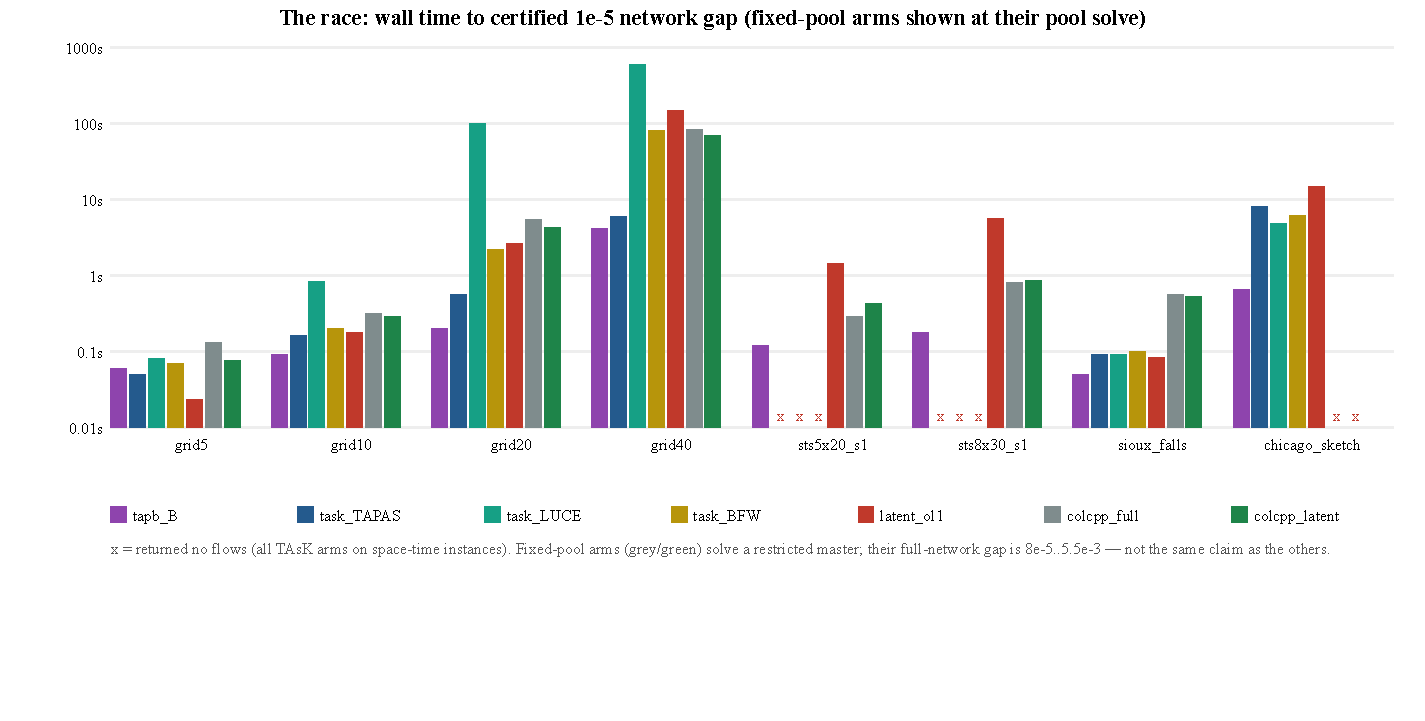
\includegraphics[width=\textwidth]{figs/chart_race.pdf}
\caption{Certified wall time to a $10^{-5}$ network gap across the
instance ladder (log scale). Crosses mark arms that returned no flows;
fixed-pool arms are visually separated because they answer a
restricted-master question (P2).}
\label{fig:race}
\end{figure}

\begin{table}[h]
\centering\small
\caption{Certified results on three representative rungs (time in seconds
to recomputed gap $\le 10^{-5}$; ``---'' = returned no flows).}
\label{tab:race}
\begin{tabular}{lrrrrr}
\toprule
Arm & grid20 & grid40 & sts $8{\times}8{\times}30$ & Sioux Falls &
Chicago Sketch \\
\midrule
Algorithm B (tap-b) & 0.20 & 4.17 & 0.18 & 0.05 & 0.65 \\
TAPAS (TAsK) & 0.57 & 6.04 & --- & 0.09 & 8.18 \\
LUCE (TAsK) & 100.14 & $>$600 & --- & 0.09 & 4.84 \\
BFW (TAsK) & 2.21 & 79.91 & --- & 0.10 & 6.20 \\
Adaptive latent GP (Python) & 2.65 & 150.27 & 5.56 & 0.08 & 14.62 \\
\bottomrule
\end{tabular}
\end{table}

\subsection{Findings}
\textbf{Bush-based methods dominate one-shot solving at scale.} On grid40
(1{,}756 nodes), Algorithm~B certifies in 4.2\,s and TAPAS in 6.0\,s while
BFW needs 79.9\,s and LUCE exhausts its 600\,s budget at
$1.7\times10^{-4}$. On Chicago Sketch, Algorithm~B certifies at
$4.3\times10^{-6}$ in 0.65\,s. TAPAS routinely converges deepest
($1.8\times10^{-7}$ on Sketch), consistent with its
paired-alternative-segment structure, at moderate extra cost.

\textbf{An origin-based sensitivity worth naming.} LUCE degrades sharply
and specifically on route-rich congested grids --- 100\,s on grid20 where
TAPAS needs 0.57\,s --- while remaining competitive on canonical networks.
Operation-level counters attribute the gap to local-problem iterations
exploding with path multiplicity; a dedicated study is scheduled.

\textbf{Only two arms survive the space--time track.} All three TAsK
algorithms return no flows on the time-expanded DAGs; Algorithm~B and the
adaptive latent-GP arm certify ($3.3\times10^{-6}$ in 0.18\,s and
$9.9\times10^{-6}$ in 5.6\,s respectively on $8{\times}8{\times}30$). For
emerging departure-time-expanded formulations, robustness --- not merely
speed --- currently separates solvers (P5).

\textbf{Runtime alone would mislead.} The Python arm's wall times reflect
its interpreter, not its algorithm --- its shortest-path call counts and
column counts are competitive, and its C++ twin (Section~7.1) removes the
language penalty. This is P6 in action: the comparison publishes work
counters next to every time.

\section{Demonstration Studies}

\subsection{Same-kernel isolation of a representation effect (P4, P7)}
Does folding an OD pair's minor paths into one aggregate column help? The
laboratory's answer isolates the representation: one C++ engine, one
$K{=}32$ pool per instance, compression toggled on and off, all else
identical. Table~\ref{tab:iso} and Figure~\ref{fig:iso} report end-to-end
effects of 1.05--1.7$\times$ (and up to 4.2$\times$ on the solve stage in
the decomposition runs), at objective errors of order $10^{-6}$ ---
essentially free in accuracy. The effect grows with path richness and
vanishes on path-poor networks where pools rarely exceed the retained-major
budget: on Chicago Sketch pools (mean depth 2.4 paths per OD), compression
is a structural no-op. A budget sweep on the adaptive arm adds the failure
boundary: over-compression (two majors on a congested route-rich grid)
fails not by inaccuracy but by \emph{churn} --- pricing regenerates the
paths the fold destroyed (43{,}778 columns generated, 20{,}333 folded,
iteration cap reached) --- so the compression budget must exceed the
equilibrium's active path multiplicity.

\begin{table}[h]
\centering\small
\caption{Atom on/off with engine and pool fixed (pool gap target
$10^{-5}$).}
\label{tab:iso}
\begin{tabular}{lrrrr}
\toprule
Instance & full GP (s) & compressed (s) & speedup & objective error \\
\midrule
grid5 & 0.130 & 0.076 & 1.7$\times$ & $3.9\times10^{-6}$ \\
grid10 & 0.316 & 0.292 & 1.1$\times$ & $2.3\times10^{-6}$ \\
grid20 & 5.49 & 4.24 & 1.3$\times$ & $2.3\times10^{-6}$ \\
grid40 & 83.0 & 69.7 & 1.2$\times$ & $1.6\times10^{-6}$ \\
Sioux Falls & 0.561 & 0.536 & 1.05$\times$ & $2.1\times10^{-7}$ \\
\bottomrule
\end{tabular}
\end{table}

\begin{figure}[h]
\centering
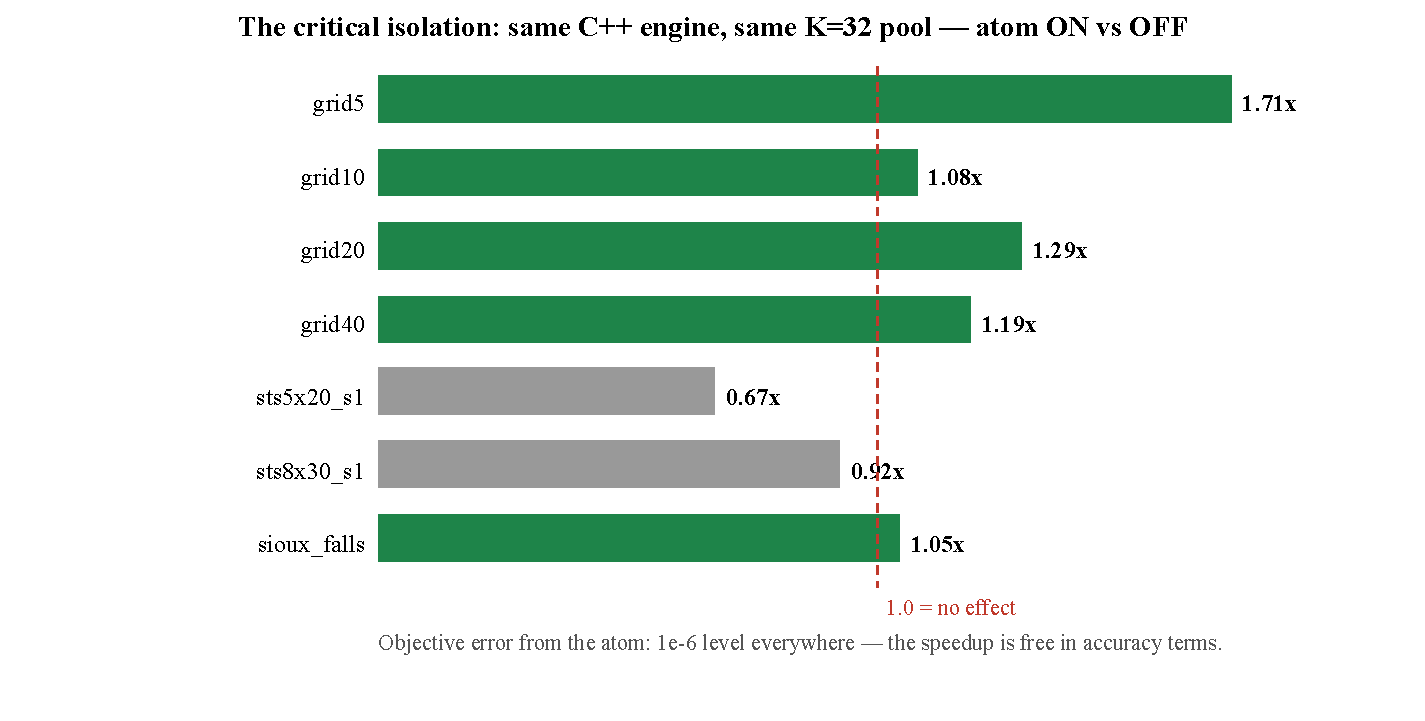
\includegraphics[width=0.85\textwidth]{figs/chart_isolation.pdf}
\caption{The same-kernel isolation chart: one engine, one pool,
representation toggled. Differences are attributable to representation
alone (P4).}
\label{fig:iso}
\end{figure}

\subsection{Restricted-pool adequacy pricing (P2)}
Every fixed-pool run in Section~7.1 reports two gaps. The pool gap reaches
$10^{-5}$ everywhere; the recomputed network gap does not: $8\times10^{-5}$
on grid5, $1.4\times10^{-3}$ on grid10, $2.3\times10^{-3}$ on grid20,
$5.5\times10^{-3}$ on grid40, and $3.6\times10^{-3}$ on Sioux Falls ---
\emph{identical for the compressed and uncompressed arms}. The pool, not
the representation, binds accuracy; compression costs nothing, and
adequacy is a property that only network-wide pricing can certify. Pools
here were generated by deterministic link-penalty $K$-shortest-path
(penalty 1.5, deduplicated by link sequence), stored in a compact binary
CSR layout so that large $K$ is affordable --- consistent with the
compressed-assignment observation that pool size need not burden the
optimizer when minor paths never become explicit variables
\citepara{Zhou et al. 2026}.

\subsection{Scenario reuse and origin templates: work-unit economics (P6,
P7)}
Two experiments locate where compressed representations actually pay.

\emph{Scenario reuse.} A base full-pool solve fixes a compressed model ---
per OD, an anchor, up to six majors ranked by nominal flow, and one column
of fixed nominal minor shares. Eight demand/capacity scenarios
($\pm$5--30\% demand, $-$10\% capacity) then re-solve warm in the
compressed space against cold full-pool re-solves, both to identical
represented-set gaps. On the route-rich grid20, compressed re-solves run
2.0--3.8$\times$ faster per scenario with the speedup \emph{growing} in
perturbation size, and cumulative cost including all setup breaks even at
scenario~4; capacity-shock scenarios benefit most. On path-poor Sioux
Falls the break-even arrives at scenario~7, and the frozen model's
objective error grows measurably with drift ($1.4\times10^{-4}$ at demand
$\times$1.3), locating the refresh threshold near $\pm$20--30\% demand
change --- a quantified design rule rather than a heuristic.

\emph{Origin-flow templates.} A second experiment tests a structurally
different object under P7: a complete feasible origin-flow template
$H\in\{x\ge0:Nx=b_o\}$ serving \emph{all} destinations of one origin, with
the origin's flow maintained as a convex combination
$x^o=\sum_j\lambda_j H_j$ --- feasible for any weights by construction.
On single-origin monotone grids with a topological-DP bush worker as the
reference (B0), fixed primed templates (L1) plateau exactly as theory
predicts --- the convex hull of $J$ templates does not contain equilibrium
($J{=}16$ spends 96 sweeps to reach only $1.6\times10^{-4}$) --- while the
adaptive variant (L2), which mints a new template from a two-sweep bush
oracle whenever the certified gap stalls, reproduces the reference solution
(objective within $10^{-6}$, certified gap under $10^{-5}$) with only two
retained templates. The economics, however, are honest and negative on
this instance class: B0 itself converges in 7--9 sweeps, leaving no sweep
budget for a latent layer to save. Combined with the scenario-reuse result,
the boundary is clear: compressed representations earn their keep where
solver work is \emph{expensive or amortized} --- scenario pipelines,
stochastic loading, time-expanded path spaces --- not in one-shot
equilibrium computation, where bush methods remain the reference. The
laboratory reports this boundary with the same prominence as the
successes (P5).

\section{Practical Applications}

\textbf{Agencies} can certify vendor or consultant solver deliverables
from returned link flows alone: the validator recomputes costs,
conservation, and the equilibrium gap in seconds and flags claims that do
not survive recomputation --- including the class of interchange defects of
Section~5, which are precisely the ones procurement reviews miss.
\textbf{Model developers} converting between GMNS, TNTP, and native
formats inherit converters in which each defect class found here is fixed
and regression-tested. \textbf{Researchers} comparing algorithms obtain an
instance ladder from hand-verifiable analytical cases to canonical and
multimodal city networks, lanes that keep restricted-pool and full-network
claims separate, and work-unit accounting that makes cross-family
comparisons meaningful. \textbf{Educators} gain exact-answer instances ---
the forged Braess network reproduces 82.25 versus 66.00 minutes at
machine precision --- and a transparent pure-Python reference solver whose
every step is readable.

\section{Conclusions and Ongoing Refinements}

This paper introduced TAPLab, an open laboratory for reproducible traffic
assignment experiments, organized around eight design principles and
demonstrated through a defect study, a certified seven-algorithm
comparison, and three protocol demonstrations. The defect study is, in the
authors' view, the sharpest argument for the laboratory: five silent
substitutions of the intended problem, in mature software, all invisible
to self-reported convergence and all caught by one inexpensive independent
recomputation. The certified comparison confirms the dominance of
bush-based equilibration for one-shot solving, quantifies an origin-based
method's sensitivity to route richness, and shows that robustness on
time-expanded networks currently separates solvers as much as speed. The
demonstrations establish where compressed path representations pay ---
rich path spaces, scenario pipelines, amortized workflows --- and where
they structurally cannot.

Scheduled refinements of the multi-year program continue along the
laboratory's roadmap: a unified C++ computational kernel with Python
bindings and cross-engine equivalence tests; origin workers for general
cyclic networks with dynamic bush maintenance; Dolan--Mor\'e performance
profiles over the full ladder with failure-aware scoring; run manifests
extended with executable hashes and hardware descriptors; and a
schedule-based transit routing track. The laboratory, its instances, its
adapters, and every number in this paper regenerate from the recorded
manifests and scripts.

\section*{Acknowledgments}
[To be added.]

\section*{Author Contributions}
The authors confirm contribution to the paper as follows --- study
conception and design: [\dots]; software and experiments: [\dots];
analysis and interpretation: [\dots]; draft preparation: [\dots]. All
authors reviewed the results and approved the final version.

\section*{References}
\begin{itemize}
\item[] Bar-Gera, H. 2002. Origin-based algorithm for the traffic
assignment problem. \textit{Transportation Science} 36 (4): 398--417.
\item[] Beiranvand, V., W. Hare, and Y. Lucet. 2017. Best practices for
comparing optimization algorithms. \textit{Optimization and Engineering}
18: 815--848.
\item[] Dial, R. B. 2006. A path-based user-equilibrium traffic assignment
algorithm that obviates path storage and enumeration.
\textit{Transportation Research Part B} 40 (10): 917--936.
\item[] Dolan, E. D., and J. J. Mor\'e. 2002. Benchmarking optimization
software with performance profiles. \textit{Mathematical Programming} 91:
201--213.
\item[] Gentile, G. 2014. Local user cost equilibrium (LUCE): a bush-based
algorithm for traffic assignment. \textit{Transportmetrica A} 10 (1):
15--54.
\item[] Gleixner, A., et al. 2021. MIPLIB 2017: data-driven compilation of
the 6th mixed-integer programming library. \textit{Mathematical Programming
Computation} 13: 443--490.
\item[] Halko, N., P.-G. Martinsson, and J. A. Tropp. 2011. Finding
structure with randomness: probabilistic algorithms for constructing
approximate matrix decompositions. \textit{SIAM Review} 53 (2): 217--288.
\item[] Jayakrishnan, R., W. K. Tsai, J. N. Prashker, and S. Rajadhyaksha.
1994. A faster path-based algorithm for traffic assignment.
\textit{Transportation Research Record} 1443: 75--83.
\item[] Perederieieva, O., M. Ehrgott, A. Raith, and J. Y. T. Wang. 2015.
A framework for and empirical study of algorithms for traffic assignment.
\textit{Computers \& Operations Research} 54: 90--107.
\item[] Xie, J., and C. Xie. 2015. Origin-based algorithms for traffic
assignment: algorithmic structure, complexity analysis, and convergence
performance. \textit{Transportation Research Record} 2498: 46--55.
\item[] Zhou, X., P. Li, Y. Liu, Y. Li, and D. Bertsekas. 2026. Compressed
traffic assignment with the augmented Lagrangian method. Preprint,
arXiv:2604.23101.
\end{itemize}

\end{document}
